%%%%%%%%%%%%%%%%%%%%%%%%%%%%%%%%%%%%%%%%%%%%%%%%%%%%%%%%%%%%%%%%%%%%%%%%%%%%%%%%
%2345678901234567890123456789012345678901234567890123456789012345678901234567890
%        1         2         3         4         5         6         7         8

%\documentclass[letterpaper, 10 pt, conference]{ieeeconf}  % Comment this line out
                                                          % if you need a4paper
\documentclass[a4paper, 10pt, conference]{ieeeconf}      % Use this line for a4
                                                          % paper

\IEEEoverridecommandlockouts                              % This command is only
                                                          % needed if you want to
                                                          % use the \thanks command
\overrideIEEEmargins
% See the \addtolength command later in the file to balance the column lengths
% on the last page of the document



% The following packages can be found on http:\\www.ctan.org
%\usepackage{graphics} % for pdf, bitmapped graphics files
%\usepackage{epsfig} % for postscript graphics files
%\usepackage{mathptmx} % assumes new font selection scheme installed
%\usepackage{times} % assumes new font selection scheme installed
%\usepackage{amsmath} % assumes amsmath package installed
%\usepackage{amssymb}  % assumes amsmath package installed
\usepackage[T1]{fontenc}
\usepackage[latin1]{inputenc}
\usepackage{graphicx}

\title{\LARGE \bf
ROSDashboard: a visual debugging tool for robotics
}

%\author{ \parbox{3 in}{\centering Huibert Kwakernaak*
%         \thanks{*Use the $\backslash$thanks command to put information here}\\
%         Faculty of Electrical Engineering, Mathematics and Computer Science\\
%         University of Twente\\
%         7500 AE Enschede, The Netherlands\\
%         {\tt\small h.kwakernaak@autsubmit.com}}
%         \hspace*{ 0.5 in}
%         \parbox{3 in}{ \centering Pradeep Misra**
%         \thanks{**The footnote marks may be inserted manually}\\
%        Department of Electrical Engineering \\
%         Wright State University\\
%         Dayton, OH 45435, USA\\
%         {\tt\small pmisra@cs.wright.edu}}
%}

\author{Felix Kaser$^{1}$, Bruce A.~MacDonald$^{2}$% <-this % stops a space
%\thanks{*This work was not supported by any organization}% <-this % stops a space
\thanks{$^{1}$F. Kaser is a student in the Software Engineering Elite Graduate Program at Universit�t Augsburg, TU M�nchen and LMU M�nchen.
        {\tt\small kaserf at in.tum.de}}%
\thanks{$^{2}$B. MacDonald is an Associate Professor at the Department of Electrical and Computer Engineering, University of Auckland,
        New Zealand
        {\tt\small b.macdonald at auckland.ac.nz}}%
}

\begin{document}

\maketitle
\thispagestyle{empty}
\pagestyle{empty}

%%%%%%%%%%%%%%%%%%%%%%%%%%%%%%%%%%%%%%%%%%%%%%%%%%%%%%%%%%%%%%%%%%%%%%%%%%%%%%%%
\begin{abstract}

Data collected during debugging is traditionally rendered as text. In object oriented languages objects are often rendered as such with their respective properties, but the final representation of data instances is still text. This might have worked out [better wording] well when normal software systems were developed, which mostly focused on user input processing. The special application field of robotics faces problems with this approach. A typical robotic system constantly gathers data from the surrounding environment through sensors. Robotic applications are also hard to interrupt during debugging, since robots generally don't run in a deterministic and suspendable environment. This paper introduces a new tool to support debugging of robotic applications. It takes into account the special needs for such a tool in a robotic development environment, especially the uninterrupted rendering of debugging data and the need for better visualization of data to support a faster interpretation of data. The goal is to support the developers understanding of data collected through the robots sensors during the development of robotic applications. A graphical user interface was developed where developers can choose their favourite visualizations for different data types.

%Debugging robotic systems is particularly complex due to the nature of data that is debugged. There is a gap between a high level data visualization tool like rviz and a low level message logging tool like rosconsole. The high level rviz tool is specialized for 3d visualization of complex data like robot arm movement, laser range data and point cloud data. rviz was not designed to visualize abstract data that is handled during the execution of a robot. Such data is often used to debug algorithms. To capture the data most developers use a printf-debugging style, often also logging frameworks. In ROS this can be achieved by using the core logging API, which sends messages containing the data to the special /rosout topic. Tools like rosconsole or rxconsole can be used to display those messages. While this data does not need complex 3d visualizations, it can still be useful to visualize the data in some way.

\end{abstract}


** I put my comments with double asterisks. 

** One general comment: about the style of the writing, it needs to be a bit more formal, less use of qualitative adjectives and cut out the words that are not adding to the key meaning of the sentence; some of the editing I did was for that ** 

%%%%%%%%%%%%%%%%%%%%%%%%%%%%%%%%%%%%%%%%%%%%%%%%%%%%%%%%%%%%%%%%%%%%%%%%%%%%%%%%
\section{INTRODUCTION}

%Debugging is a complex topic, especially for robotic systems where the developer needs not only to deal with code complexity but also with a distributed environment. There are many different frameworks and hardware approaches, a standard is hard to define. Due to the complexity and the diversity of frameworks and hardware many developers build their own tools to assist them in the development and debugging of their applications\cite{Collett2010}.

%When debugging a robot a developer usually faces two main challenges: data acquisition and data visualization. This paper introduces a new tool for data visualization in robot applications and will shortly present different approaches to data acquisition. The goal of the tool is to improve the visualization of debugging data and give developers a generalized tool that can be easily adapted to different robot applications.

%Data acquisition has been addressed in previous work by Gumbley, where a framework was introduced to gather debugging data without interrupting the execution of a robot application\cite{Gumbley2009}.

Current debugging tools for robotics are mostly based on debugging techniques and interfaces developed for traditional non-robotic applications. Those techniques and interfaces were developed specifically to suit the requirements of traditional systems: handling arbitrary and abstract data. Since then the computing world has changed, but many developers still have to use tools which were developed under different circumstances and based on different requirements. Especially robotic applications are different from traditional systems, because the data they handle are not as arbitrary and abstract as in traditional systems. Robots need to handle data that closely relates to the real world and the perception of the robot. The main data source for robots are its sensors which provide a continuous data stream whereas in many traditional systems the data is discrete and based on user input. This raises new requirements for debugging tools and makes many traditional tools hard to use within the field of robotics.

We need better debugging tools to handle the special kind of data in robotics. Traditional debugging tools usually render data collected during debugging as text. Under the debugging circumstances of a traditional system this was not a big problem, because the execution of the program was interrupted and the developer had enough time to interpret and understand the data. When debugging robotic applications this can be a problem, because of the nature of the application: Robotic applications usually can not be interrupted in their execution, because robots generally don't run in a deterministic and suspendable environment \cite{Gumbley2009}. Interrupting a robotic application would destroy the continuity in which the sensors collect data, the environment of the robot would change substantially and the situation in which the application was debugged changed. Some technical solutions have been presented in recent years \cite{Gumbley2009}, but many developers still rely on printf-style debugging or other logging mechanisms to collect data without interrupting the execution of the program. The problem with data collected this way is the text-only nature of data, which requires the developer to constantly parse and interpret logging messages which often contain more complex content like numbers.

While most of the currently available visualization tools focus on spacial data to help understand the robot and the runtime environment \cite{Collett2010, Collett2007, Collett2006, Quigley2009}, rendering of abstract data is still uncommon. This paper presents a tool to visualize abstract data to support the developer with problem detection and debugging. In past research visualization has been successfully used to reduce the cognitive effort to understand the structure of a computer program \cite{Tudoreanu2003}, with the tool presented in this paper a first step towards the evaluation of the impact of data visualization on the cognitive effort during debugging has been made.
% [next part is experimental] The tool presented in this paper tries to apply the same principles to debugging. [Hypothesis:] Visualizing data in a way that fits the developers expectations and mental model reduces the cognitive effort needed to understand the data [cite!]. Using visualizations during the debugging process can help developers to interpret and understand the data much faster [this is actually the hypothesis, still to be evaluated in the future], without the need of interrupting the execution of a robot application.

Another problem when debugging robots is that existing debugging tools often don't support developers and researchers of robotic applications enough. As a result many develop their own tools that suit their application area and problem statement best \cite{Collett2006}. Developing your own debugging tool is extremely time consuming and the developed tools are often one-time-only tools, because they don't fit the use case of other applications and are too hard to adapt to a new project.

[should I mention the specifics like ros topics and that our tool connects logging statements in the source code with a visualization widgets on a dashboard? I've tried not to dig into details already, but it might not explain what we are exactly doing (yet)]

ROSDashboard, the tool presented in this paper, is designed for robot development in general and not specific to one application area. The goal was to create a visualization tool that can be used for many different robot applications and is easy to adapt, in case developers want to use it for a specific use case where the default implementation is not sufficient. ROSDashboard provides a dashboard interface to robot developers, which they can populate with graphical widgets to visualize data from the robot. The dashboard can be customized to display widgets according to the current robot hardware and development stage. It can be used to visualize data during debugging as well as monitor data during the normal execution of the robot. This means ROSDashboard is a tool that a) can be adapted to many different use cases and b) allows the developer to choose the widgets he thinks represent the data best, according to their mental model and the meaning of the data. The tool is based on ROS (Robot Operating System) which abstracts from specific robot hardware and takes care of inter process communication \cite{Quigley2009}. ROS has a significant community backing the project and supports many of the currently available robots \cite{Foote2012}.

%Developers face a different set of challenges when developing and debugging robotic systems instead of traditional software systems \cite{Collett2010, Collett2006, Gumbley2009}. Debugging is a complex task that generally consists of data acquisition and data visualization.
%In traditional software systems the data visualization is mostly rendered text. Although it might not be the best representation for data, text definitely is the most unified representation and is therefore a good choice for traditional software systems that deal with every kind of data.
%When developing applications for robots, this proves to be a challenge. Robots usually handle sensory data which is highly related to the environment where the robot operates. Traditionally this data is represented as text. This paper presents a new approach to visualize simple data when debugging a robot. Current solutions and problems with those solutions are outlined and a new tool is introduced to take care of the data visualization.

%Interpreting and understanding debugging data is much faster if the data is represented in a way that a) is natural in respect to the type of data and b) fits the mental model of the developer. Some research has been conducted in the direction of augmented reality (AR) debugging \cite{Collett2006, Collett2010}. Augmented reality debugging [tries to?] bridges the gap in the perception of the world from a human (developer) point of view and a robot point of view. ARDev, the system introduced in \cite{Collett2010} only focuses on visual representation of global perception data like laser-range data, path visualizations, ...
%The tool presented in this paper addresses visualization of abstract data, which was identified as possible future work in \cite{Collett2010}.

%The field of robotics consists of really diverse hardware solutions for different kinds of problems. This lead to high number of frameworks and tools for robot development without a clear standard. Due to the complexity and the diversity of frameworks and hardware many developers build their own tools to assist them in the development and debugging of their applications\cite{Collett2010}, which contributes even more to the fragmentation of frameworks and tools.
%The goal for the tool presented in this work was to be customizable and adaptable to different kinds of robots and projects, in order to be a useful tool to as many developers as possible. This was one of the main requirements and is described in more detail in section \ref{requirements}.

%Data acquisition in robotic environments is difficult due to ``the robot environment, the inherent nature of mobile robots, and the nature of mobile robot tasks''\cite{Collett2010}. [wrong citation, does not refer to data acquisition]

% Debugging robotic systems has proven to be more difficult than debugging generic computer systems [check citation!] \cite{Collett2010}. Developers face the challenge of data acquisition and data visualization. Acquiring data in a robot environment can be difficult because normal debugging approaches such as breakpoints are infeasible, because interrupting the robot during runtime can alter the state of the robot in a way that 

% One of the biggest problems when debugging robotic systems is the non-interruptible nature of robotic applications. Sometimes it is hard or even impossible to interrupt the execution of a robot without the danger of damaging the robot hardware or putting the people in the surroundings at risk. ** need to be more specific than ``threat''; what exactly do you mean? ++ better? ** For example you can not just interrupt a quad-copter in mid-flight to step through the algorithm to find a bug. [citation? rewrite? drop the example?]

%One approach is to design two separate controllers: a low level controller that keeps the essential parts of the robot running (e.g. keep the quad-copter flying) and a high level controller that runs the application logic code which is debugged. This only solves part of the problem because developing the low level controller is still not interruptible. [citation?] and because the application logic may need to respond to external inputs at any time.

%---> this could go into related work (data acquisition)
%Another approach is the concept of tracepoints for debugging a robot application without interrupting the execution but analysing the trace either after the application finishes, or viewing the results live \cite{Gumbley2009}. Tracepoints are a highly instrumented way of debugging and do not require modifications to the source code.
%A less instrumented method of debugging still used by many developers [no numbers to prove that, could not find any studies] is so called printf-debugging. Print statements are used to collect and output values during the execution of a program which can be viewed either live or after the application finished. Using printf-debugging is highly flexible and easy but it requires source code modifications and it can be difficult to keep track of print statements in bigger applications. In higher languages (and frameworks) this method is often supported by tools and can be refactored out of release compilation units for optimization. [for example android logcat and log4j in general, should I be more specific?]

%One issue that still remains with all of the above methods is the representation of data. All of the methods represent data as text and it can be [it is? whats the correct wording here?] hard to interpret the different values. [@ bruce: OK this needs some work, I'm trying to write down what I would like to express, maybe you can help me to find better (more scientific) words for it or tell me to drop it completely]. Interpreting and understanding data is much faster if the data is represented in a way that a) is natural in resprect to the type of data and b) fits the mental model of the developer. Some research has been conducted in the direction of augmented reality (AR) debugging \cite{Collett2006} \cite{Collett2010}. Augmented reality debugging [tries to?] bridges the gap in the perception of the world from a human (developer) point of view and a robot point of view. ARDev, the system introduced in \cite{Collett2010} only focuses on visual representation of global perception data (laser data, path visualizations, ...) and visualization of abstract data was identified as possible future work in \cite{Collett2010}.

%This paper presents a new tool to visualize abstract and algorithm-local data: ROSDashboard. The tool visualizes data collected with a printf-style approach [how do I say that printf-style was chosen because it was the fastest way to access data for the prototype? Should I drop it here and write about it in the requirements/design?] and the developer can arrange widgets on a dashboard to visualize the debugged data in a more natural way. The developer can choose which visualization he or she prefers and best suits his or her mental model of the data. The goal of the tool is to further improve debugging data visualization and debugging in general.
%[drop next sentence]However the tracepoint approach is complex and pre-execution configuration takes a substantial effort and skill, which many developers won't like to take upon them. [badly written, rewrite, no proof** I tried to improve the writing; however I agree there is no proof of the substantial effort and I don't believe it either! need to be more precise and exact about the issues]

%[@ bruce: I am thinking of dropping this paragraph in favour of a different approach (the one above)]Because of the problems stated above many developers still use printf-debugging [proof?] It is something they can use with the skills they already have, without learning a new toolset and setting up a tracing or debugging chain[proof?]. One major downside of printf-style-debugging is the text-only representation of data. Although the developers might be used to looking at and interpreting numbers scrolling down in a console window, it is not a very natural representation of the data. This paper [we or I? ** neither unless its important to the argument; just stick with the info to be presented, as I changed it to **] presents a new approach to improve printf-style-debugging with a new tool: ROSDashboard. The tool visualizes data collected with a printf-style approach and the developer can arrange widgets on a dashboard that visualize the debugged data in a more natural way. The developer can choose which visualization he or she prefers and best suits his or her mental model of the data. [unnecessary?: While printf-debugging has its downsides, there are also benefits to printf-debugging. The developer knows exactly where the printf-statements are and this makes it easy to understand the flow of a program.]


** Goal of the work needs to be stated concretely and specifically; something clear and strong. Did the proposal provide that? Else there is nothing to hang the background and requirements on ** [is this better now?]

\section{RELATED WORK}

\subsection{ROS - Robot Operating System}

** Suggest this is a background about debugging in robotics; what is the history there? it isn't coming through here. Does Collett have anything to say about it? **

%** this next bit is not really relevant to the paper; why not talk about its debugging capabilities **
%The first work on ROS was done as part of the STanford Artificial Intelligence Robot (STAIR) in 2007 \cite{Quigley2007}. The original software library was called \emph{Switchyard} and had been developed at Stanford. Later the library was refined and generalized to also suit the requirements of the Personal Robot Program at Willow Garage\footnote{www.willowgarage.com} \cite{Quigley2009}. The resulting general framework has been released as Open Source \cite{Quigley2009} and a community of researchers and industry partners has grown that supports and keeps developing the framework.
%** previous bit is not so relevant here **

** This paragraph is more relevant I think. I think it needs some addition to explain why its relevant and how it relates to debugging **
ROS is an Open Source framework for complex robotic systems. It was developed to abstract from the hardware of the robot and make it easier to create modular robot software, which can run on different robots and on different machines. The modular approach makes development easier because it can be divided amongst different developers or development teams. This also allows it to exchange only small parts of a complex system, without the need to redeploy build and re-deploy the whole system.
The modules in ROS are called \emph{nodes} and several nodes executed together are called a \emph{stack}. ROS \emph{packages} bundle nodes and stacks and are used to make software modules available to other developers. Everyone can create their own package which can be indexed by ROS so that your software modules can be found, downloaded and used by other developers. There exist many packages, nodes and stacks with implementations of algorithms for some of the most common problems in robotics (e.g. navigation, localization, joint movement, etc.) and they can easily be (re-)used.

%When an application is not running as expected, this is usually due to a problem in the composition of the modules or a local problem in one of the modules. For both categories there are several tools that allow developers to investigate the problem:
%Several tools have been developed for ROS to assist developers during debugging. Some of the tools are console based and can be used to inspect the various messages transmitted on topics. Other tools are graphical tools to visualize 
ROS comes with several tools to assist the developers during the development and debugging of a robot. The tools most relevant to this work are:
\begin{description}[\setlabelwidth{rxconsole}]
%\item[rxgraph] is a graphical tool based on the command line tool rosgraph. It visualizes how modules are connected to each other and with which topics they communicate.
\item[rostopic] a command line tool to monitor topics and emit messages to topics.
\item[rxplot] a graphical tool which plots data from one or more topic fields on a cartesian coordinate system.
\item[rxconsole] displays logging messages that have been emitted on the special purpose topic /rosout.
\item[rviz] renders models of the robot in 3d and visualizes spacial data like point clouds, robot poses and trajectories, etc. \cite{Quigley2009}.
\end{description}

The tool presented in this paper fills the gap between a textual representation of data (rostopic, rxconsole) and a highly sophisticated 3d visualization of spacial data (rviz). rxplot is already positioned in between the textual and 3d visualization tools, but it offers only one form of visualization: a time graph.

%rostopic and rxconsole display logging messages as text. Their purpose is not to visualize data but to assist the developer during the development as a logging framework. rxplot is designed to visualize data on a cartesian coordinate system, which is mostly useful for measurements and not for data visualization. rx
%rviz was created because it is extremely hard to understand what is going on in the robots environment by only looking at numbers. --> point out that more abstract data is not visualized at all, thus the need for rosdashboard.

** again, state the relevance to debugging **
The communication between ROS nodes can be done asynchronously through a publish/subscribe mechanism and synchronously through services. Nodes can send messages by publishing a message on a topic and receive messages by subscribing to that topic. This mechanism is flexible and decouples the sender from the receiver. A publisher node does not need to know if there are other nodes listening and vice versa. For synchronous communication and guaranteed delivery of messages, services can be invoked. The routing is established during runtime through the ROS core. The core of ROS was kept really slim and only contains the most essential parts of the framework (such as the inter node communication). ROS can run on several machines distributed in a network, the only restriction is that every node needs to know the address of the core (master node) in order to communicate with other nodes.

The ROS communication structure is used by ROSDashboard to connect the logging statements in the source code with the visualization on the dashboard. This allows to re-use existing data streams published on topics without introducing changes to the source code. If new data needs to be collected, the source code needs to be modified to publish the data on a topic.

\subsection{LabVIEW}

** need to include more about the relevance **

LabVIEW (Laboratory Virtual Instrumentation Engineering Workbench) is a graphical programming environment developed by National Instruments\footnote{www.ni.com}. It features \emph{Front Panels} which allows a developer to add widgets to a panel. These widgets can display the status of the graphical program or act as controls (button, knobs, etc.) for the program. For each widget on the front panel an element is created in the block diagram of the program which can be connected to other parts in the block diagram. This makes it easy to connect data source widgets (e.g. buttons) with the program and also program data with corresponding data sink widgets (e.g. graph displays). LabVIEW's front panel feature allows developers to easily create their own interfaces for a program, including visualization of abstract data in form of graphical widgets.

The front panel feature was described as ``LabVIEW's `biggest advantage', its `best feature', or its `main power' '' in the open-format answers of a survey of LabVIEW programmers \cite{Whitley2001}. The researchers concluded that the front panel (among other features) could be responsible for a large share of LabVIEW's impact, but more research is needed \cite{Whitley2001}. While this does not justify the development of a visualization tool, it shows the potential of such a feature and shows that more research needs to be done to evaluate the benefits of a visualization tool for simple abstract data.

\subsection{Tracepoints}

[this subsection either needs to become better or needs to go, it is not really relevant but I mentioned tracepoints in the introduction]

Tracepoints have been investigated as a new way of collecting data during debugging \cite{Gumbley2009}. Although tracepoints could be a data provider for a visualization tool like ROSDashboard, for the scope of the first iteration of the tool we decided to use logging statements to collect data. The existing ROS logging framework was used to collect data, because no configuration overhead is needed.

** Well you mentioned them above?? In any case, the background section should explain the background to robot debugging, so that we know what it is all about. Did you have more in the proposal; I can't remember? **

\subsection{ARDev}

ARDev is an augmented reality (AR) debugging system, developed to provide AR visualization of data during robot development \cite{Collett2010, Collett2007, Collett2006}. The AR approach to debugging helps the developer to understand the \emph{global} state of the robot by augmenting a video feed of the robot with information of the robots' perception. Initial evaluation studies were promising that the visualization can help developers significantly during debugging \cite{Collett2010}. Visualizing abstract data was identified as a potential extension to ARDev \cite{Collett2010}.

% ROSDashboard mainly focuses on the \emph{local} state of a robot application or a specific algorithm. In the future those two tools could be combined to create a better debugging tool that helps the developer on a \emph{global} as well as a \emph{local} scale.

\section{ROSDASHBOARD}

\begin{figure}[thpb]
  \centering
  \framebox{
    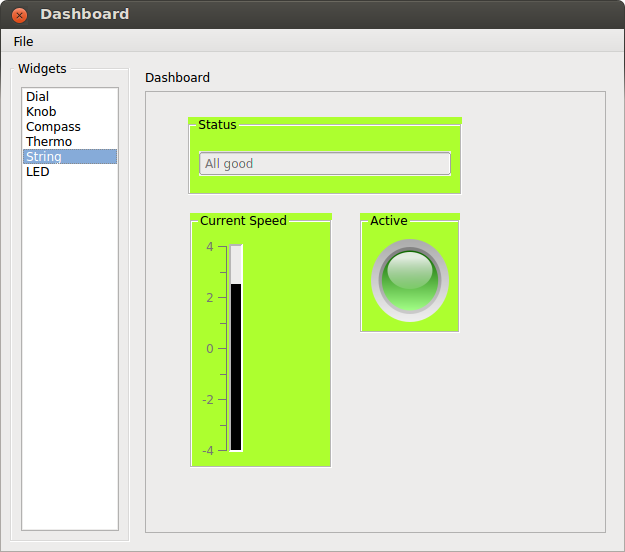
\includegraphics[scale=0.35]{images/rosdashboard_screenshot.png}
  }  
  \caption{Screenshot of ROSDashboard in action. [where should this figure go? introduction? ** no should be where you talk about the design and implementation.]}
  \label{screenshot}
\end{figure}

\subsection{Overview}
ROSDashboard is a new tool in the ROS environment. It is built to allow developers easy visualization of data streams. It is built around a central dashboard where developers can add visualization widgets with drag and drop from a toolbox. Currently there are only the most basic widgets implemented to visualize data. In future there should be added more and more widgets. This effort could come from the robot developers themselves through a simple plugin mechanism. The developers know best what widgets they need to visualize their data.

\subsection{Requirements}
\label{requirements}
** Section is pretty weak. Maybe refer back to the proposal and give clear and strong list of requirements; and they should be argued from the original goals of the work. And so the goal needs to be stated clearly and strongly above at the start.**

Requirements (easy to install and use, simple to extend, base tool for further development and evaluation)

[the requirements below are all quite high-level. should I add requirements like distributed debugging, uninterrupted debugging? they affected the design but distributed debugging is completely in ROS hands (it still affected the decision to go with ROS) ** yes, somewhere list them and say that ROS provides them. It is important here to explain the options and reasoning for design decisions. ** ]

\subsubsection{Openness}
One of the requirements is to be open. Open in terms of Open Source but also regarding the other requirements like extendibility and adaptability. Openness helps to spread the word and gain a higher user base faster. [citation?] [badly written. rewrite. ** yes need to be clear and precise and relevant. ]
\subsubsection{Low configuration overhead}
The goal was to create a useful tool that is easy to use and can be used by anyone without much configuration, setup or learning overhead. This contributes to a high user acceptance and a low entrance barrier [better wording?] for new users.
\subsubsection{Extendibility and adaptability}
Especially in robotics common standards are not yet defined and the variety of tools, frameworks and robot hardware is big. This means that the developed tool needs to be highly flexible. It should be easy to adapt the current system to work with any robot hardware supported by ROS and it should be designed with an open mind towards other frameworks. It also needs to be easy to reflect possible changes in the framework and underlying tools.
\subsubsection{Follow the ROS philosophy [really?]}
ROS is designed to have a really small core with as many tools build around the common core as needed. The principle is to have small tools that do one thing only but are really specialized and sophisticated in what they handle. This philosophy is followed and encouraged by the ROS core developers. It is important to follow this principle to reach a high acceptance among the ROS community and to fit in as good as possible with other tools.
\subsubsection{Integrable}
[explain current efforts of RQT and that rosdashboard should become part of it to be in the graphical ROS toolchain, but it was a moving target thus the integration is not done yet]
\subsubsection{Customization [flexibility?]}
Different developers prefer to visualize their data differently and every project is different. It is important [why important?] to create a system that can be customized by a developer to suit their preference and the targeted project best. [extend?] [put in citation from collett \cite{Collett2007}]


\subsection{Design}

** needs to be tied to requirements in part and then other decisions. **

Python was chosen for ROSDashboard as target language, because it is a good match for fast prototyping and iterative development. Python's duck typing [reference] turned out to be a big help for topic introspection (see implementation details \ref{topic introspection}). Qt is used for the graphical part of the tool which also reflects the general policy in the ROS community (before Qt wxWidgets was the graphical toolkit of choice). [as of 2012, look for a reference in the wiki?]

Although the current software does not support third party widgets (in form of plugins) yet, the structure of the internal widgets is aligned to allow easy integration of such a feature in the near future. For now if a third party wants to have specialized widgets, it needs to modify the source code and add the code for widgets directly to the source tree.

ROSDashboard was developed as Open Source from the very beginning to allow external contributions and feedback. The source code is hosted on Github\footnote{http://github.com/kaserf/rosdashboard}. A prototype was announced to the ROS community and valuable feedback was gathered and documented. One of the most valuable feedback was to make ROSDashboard more generic and allow to visualize topics that publish String messages which are parsed to get the data for the visualization. This would make it possible to use ROSDashboard with existing projects that already contain extensive logging (but in text form). [move the feedback to future work section, it is not really something for the design section]

\subsection{Implementation details}

** Jumps in to details that the reader cannot see relevance for completely. The details looks good and I think this could be a strong section; just needs to be related to the sections above, goal, requirements etc. Should be derived from the design section. You could have an architecture diagram, and tie it together with that. Probably start above with the ROS model, and discuss how the debugging tool requirements fit with it. Currently these things are not clear. **

\subsubsection{Topic introspection}
\label{topic introspection}
ROS topics were originally not designed and developed as something the user or developer chooses graphically. Topics are usually set up in the code. ROSDashboard exposes the topic setup in a graphical user interface and this turned out to become a challenge since one of the requirements is to have a low configuration overhead (see requirements section [add reference]). Normally you have to select a topic name and a message data type. The data type can be one of the standard message types (wrapping the basic types like Float, Integer, String and Boolean) or a more complex message type. To access one data element of a message the "datafield" field was introduced in the graphical interface. Figure \ref{topic setup screenshot} shows an exemplary topic setup configuration to access the linear velocity of the \emph{/turtlesim/Velocity} message published to the topic \emph{/turtle1/command\_velocity}. Using Pythons duck typing and the \emph{rostopic} module it was possible to avoid the complexity of dynamically binding message types during runtime and detect the message type automatically. If a topic is not yet published (and thus the message type is not defined yet) the call to \emph{rostopic} blocks until the message type becomes known. To avoid blocking of the user interface a listener thread was implemented to wait until a topic (message type) becomes available. Avoiding to manually ask the user for a message type makes the configuration of widgets easier and faster for the user and also keeps the implementation simpler (no dynamic binding of message type classes during runtime).

\begin{figure}[thpb]
  \centering
  \framebox{
    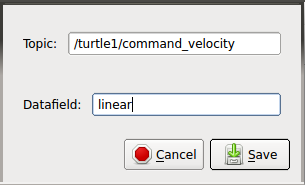
\includegraphics[scale=0.5]{images/topic_setup.png}
  }  
  \caption{Screenshot of the topic setup dialog.}
  \label{topic setup screenshot}
\end{figure}

The initial prototype implementation of the topic selection mechanism was developed to allow a fast and easy setup of widgets on the dashboard. In future the topic selection needs a better user interface to make it simpler to choose a topic and a datafield (and maybe the topic message type, if the topic introspection becomes to complicated). One possible solution could be a drop-down list with type-ahead auto completion and a visual representation of the message type and which fields are available to select. [highly opinionated paragraph. not sure if it makes sense to mention this]

\begin{figure}[thpb]
  \centering
  \framebox{
    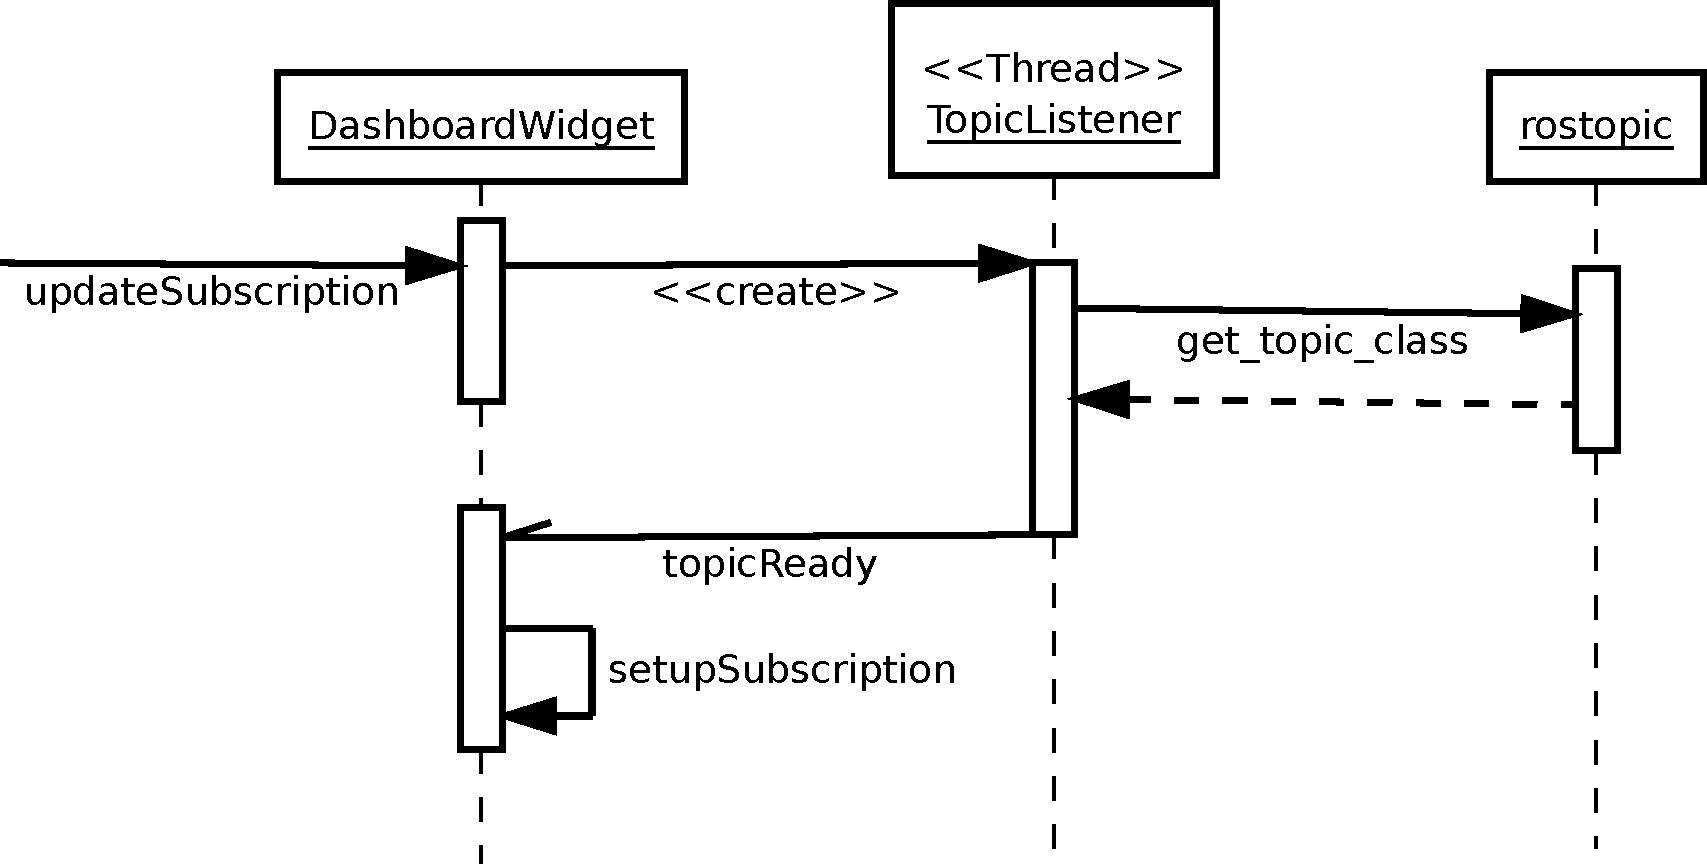
\includegraphics[scale=0.28]{diagrams/topic_subscription.pdf}
  }  
  \caption{Exemplary flow of events for updating the topic setting of a widget.}
  \label{topic subscription}
\end{figure}

\subsubsection{Object model}
The object model was designed to make it easy to extend ROSDashboard with more widgets. The abstract \texttt{DashboardWidget} class covers the general tasks that are the same for every widget. It provides hooks to overwrite some methods in the subclass if a widget needs to be more specific. This should allow easy integration of a plugin framework at [at? in? on?] a later stage, where third party widget developers only need to implement the specific parts of a new widget and the common tasks can be handled by the default implementation in \texttt{DashboardWidget}.

\begin{figure}[thpb]
  \centering
  \framebox{
    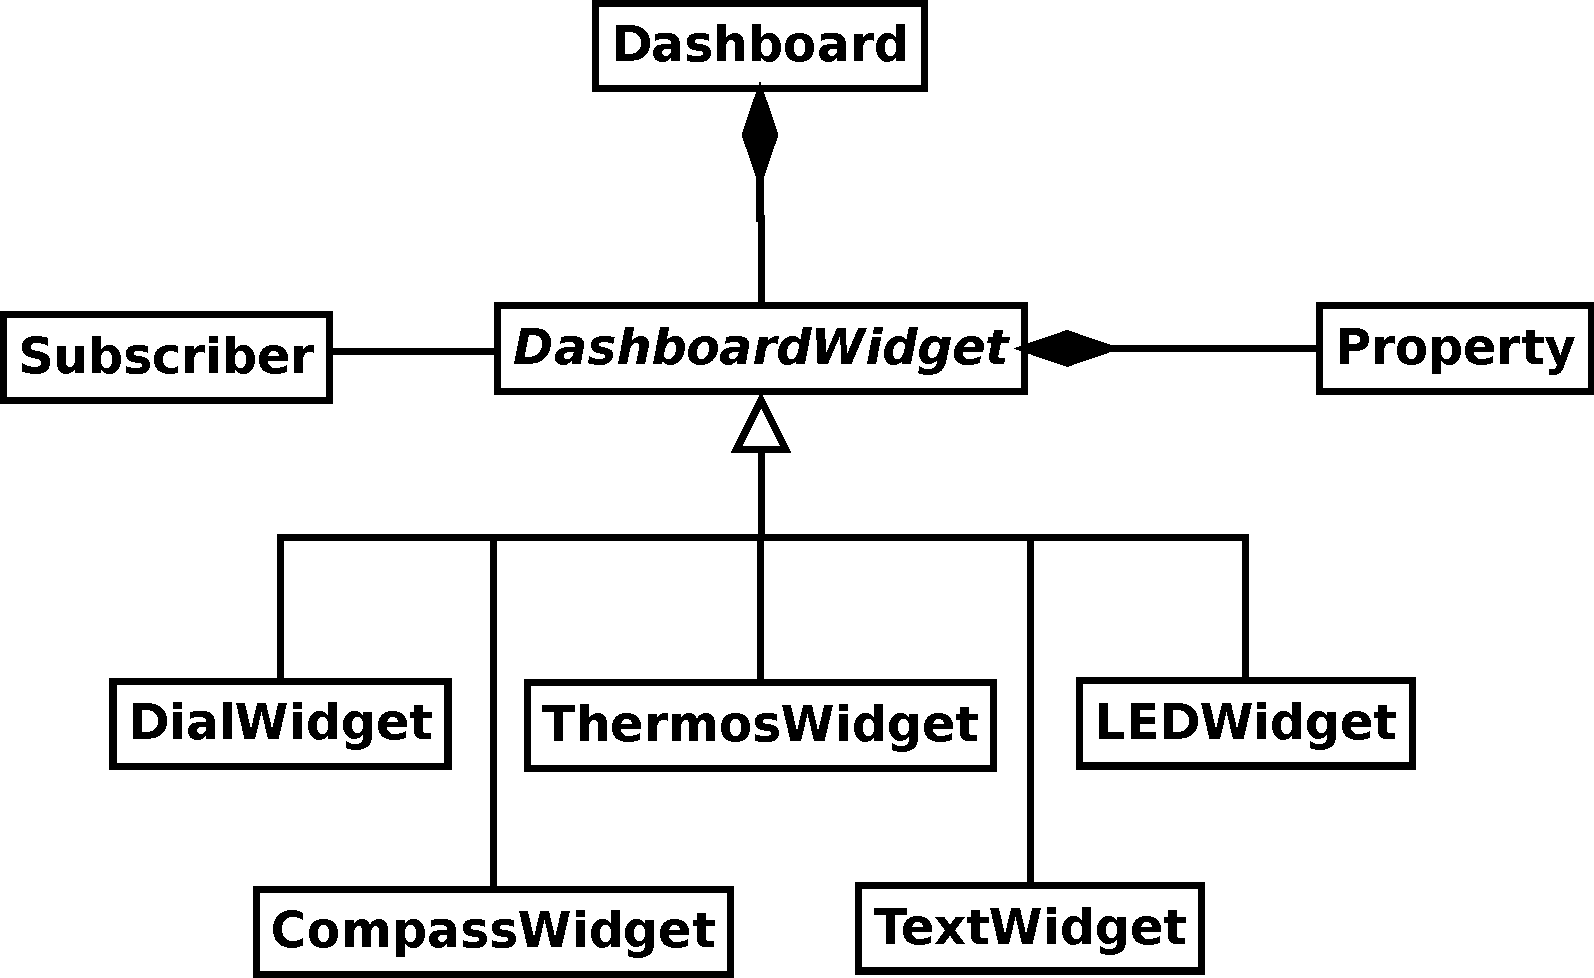
\includegraphics[scale=0.3]{diagrams/class_overview.pdf}
  }  
  \caption{Overview of the core object model structure.}
  \label{class overview}
\end{figure}

The subscription setup and the properties management are implemented in the \texttt{DashboardWidget} class as well. The main reason is to hide the technical details away from a third party plugin developer to make his life easier. The plugin developer only needs to specify which properties his widget needs and needs to implement the callback that gets called when the properties have been changed. The \texttt{DashboardWidget} supports numeric, text and float properties. If more specific properties are needed the plugin can overwrite the whole properties part and not re-use the default implementation from \texttt{DashboardWidget}.

\section{FUTURE WORK}

The presented tool is fully functional and is ready to be released. On a software side of things further work can be done to improve the number of available widgets. Ultimately this should be done through a plugin engine where third party developers can easily add widgets for new and more complex kind of data. The extendibility of the tool was one of the initial requirements and the structure of the program allows easy integration of such a plugin engine. A more long term plan for the project is to implement a parser that can extract data which is embedded in text-based messages through regular expressions. Another long term plan is to generalize the widgets to have both subscription widgets and publisher widgets. This would give developers the ability not only to monitor values during execution but also manipulate configuration values and give commands to the robot during a debugging session.

RQT is a graphical interface that groups together many different graphical tools for ROS. It was under active development during the time of this project and it was chosen not to integrate ROSDashboard into RQT yet, but to keep it in mind for future work. The plugin interfaces to integrate a tool into RQT have been finalized recently and ROSDashboard can easily be integrated. This would allow developers to use ROSDashboard amongst other graphical tools in one unified graphical interface that saves the state of all tools when exited and work can be resumed where left of.

ROSDashboard provides a good base to conduct research on the impact of visualizations during debugging of robotic applications. Future research can evaluate how visualizations affect the developer during debugging, especially if it decreases the cognitive load and thus makes debugging with visualizations faster and more productive.

\section{CONCLUSIONS}

ROSDashboard, the tool presented in this paper is capable of visualizing simple abstract data that is being published on a topic in the ROS communication middleware. Although the tool presented in this work has not been fully evaluated yet, it shows the possibilities and potential of simple visualizations during debugging or robotic applications. Further evaluations need to be conducted in order to quantify the improvements the tool has on a reduced cognitive effort and thus debugging performance.

The modular approach followed during the design of the tool makes it easy to extend and adapt the tool in the future. It also allows developers to choose a representation of data they find most helpful, with the only restriction being the number of available widgets and the data type compatibility. The simple drag and drop principle to add and remove widgets on the dashboard makes the tool flexible towards changes during the debugging process. The feature to save and restore dashboard configurations makes it easy to distribute dashboards amongst the developers. This feature can also be used to provide monitoring dashboards that can be created by robot hardware manufacturers and given out to developers.

\addtolength{\textheight}{-12cm}   % This command serves to balance the column lengths
                                  % on the last page of the document manually. It shortens
                                  % the textheight of the last page by a suitable amount.
                                  % This command does not take effect until the next page
                                  % so it should come on the page before the last. Make
                                  % sure that you do not shorten the textheight too much.

%%%%%%%%%%%%%%%%%%%%%%%%%%%%%%%%%%%%%%%%%%%%%%%%%%%%%%%%%%%%%%%%%%%%%%%%%%%%%%%%



%%%%%%%%%%%%%%%%%%%%%%%%%%%%%%%%%%%%%%%%%%%%%%%%%%%%%%%%%%%%%%%%%%%%%%%%%%%%%%%%



%%%%%%%%%%%%%%%%%%%%%%%%%%%%%%%%%%%%%%%%%%%%%%%%%%%%%%%%%%%%%%%%%%%%%%%%%%%%%%%%

\section*{ACKNOWLEDGMENT}

This work is part of the final project in the Software Engineering Elite Graduate Program at Universit�t Augsburg, TU M�nchen and LMU M�nchen\footnote{www.studieren.se}. It was conducted at the Department of Electrical and Computer Engineering, University of Auckland, New Zealand.


%%%%%%%%%%%%%%%%%%%%%%%%%%%%%%%%%%%%%%%%%%%%%%%%%%%%%%%%%%%%%%%%%%%%%%%%%%%%%%%%

%%%%% references %%%%%
\bibliographystyle{IEEEtranBST/IEEEtran}
\bibliography{bibtex/Master_Thesis,bibtex/manual}

\end{document}
